\chapter{Range-clone}
\label{chap:clone}

This chapter describes another \bet operation, range-clone, which can be used
to implement file or directory clones and renames on full-path-indexed \betrfs.
Unlikely a range-rename, which completes all its work at once, a range-clone
injects a new type of message, the \goto messages, to the \bet.
The \bet then flushes \goto messages with other messages in batches, gradually
finishing the range-clone works.
Therefore, range-clone fits into the write-optimized framework of \bets.

This chapter first describes the range-clone interface,
followed by how range-clones are implemented on \bets.
At last, this chapter describes a new technique, preferential splitting, which
makes range-clones more efficient.

\section{The range-clone interface}

\begin{table}[t]
    \centering
    \begin{tabular}{c | l}
        \hline
        Type of File System Operation & Key/Value Store Operations \\
        \hline
        \hline
        File Rename & \mdb$\rightarrow$put(\textit{dst}); \\
                    & \mdb$\rightarrow$del(\textit{src}); \\
                    & \ddb$\rightarrow$range-clone(\textit{src}, \textit{dst}, true); \\
        \hline
        Directory Rename & \mdb$\rightarrow$put(\textit{dst}); \\
                         & \mdb$\rightarrow$del(\textit{src}); \\
                         & \mdb$\rightarrow$range-clone(\textit{src/}, \textit{dst/}, true); \\
                         & \ddb$\rightarrow$range-clone(\textit{src/}, \textit{dst/}, true); \\
        \hline
        File Clone  & \mdb$\rightarrow$put(\textit{dst}); \\
                    & \ddb$\rightarrow$range-clone(\textit{src}, \textit{dst}, false); \\
        \hline
        Directory Clone  & \mdb$\rightarrow$put(\textit{dst}); \\
                         & \mdb$\rightarrow$range-clone(\textit{src/}, \textit{dst/}, false); \\
                         & \ddb$\rightarrow$range-clone(\textit{src/}, \textit{dst/}, false); \\
        \hline
    \end{tabular}
    \caption[File system renames and clones in \betrfs with range-clones]{\label{tab:fsrc}
        \betrfs renames or clones \textit{src} to \textit{dst} by calling range-clones.}
\end{table}

Similar to range-rename, range-clone is defined as:
range-clone(\spre, \dpre, \delold), where \delold is a boolean.
It does the following things:
\begin{itemize}
\item it deletes all destination key/value pairs from the key/value store;
\item then, for any source key/value pair $(k,v)$ in the key/value store,
it inserts a key/value pair $(k',v)$ to the key/value store,
where $k$ is the concatenation of \spre and some suffix $s$ and $k'$ is the
concatenation of \dpre and the same suffix $s$;
\item if \delold is true, it deletes all source key/value pairs from the
key/value store.
\end{itemize}
If \delold is true, range-clone is equivalent to range-rename;
otherwise, range-clone is range-rename without deleting source key/value pairs.
Therefore, as summarized in Table~\ref{tab:fsrc},
file or directory renames on full-path-indexed \betrfs can be done
with range-clones just as they are done with range-renames.
And clones on full-path-index \betrfs are done in the similar ways with \delold
set to false.

\section{The range-clone operation}

This section shows the implementation of range-clone operations.
Because deleting source key/value pairs can be done by injecting a range-delete
message into the root node,
\delold is set to false in the section.

This section first describes a simple range-clone implementation based on the
range-rename implementation,
followed by the technique to finish tree surgery work in flushes.
At last, this section introduces \goto messages that further write-optimizes
the range-clone operation.

\subsection{A range-clone based on range-rename}

\begin{figure}
    \begin{subfigure}{\textwidth}
        \centering
        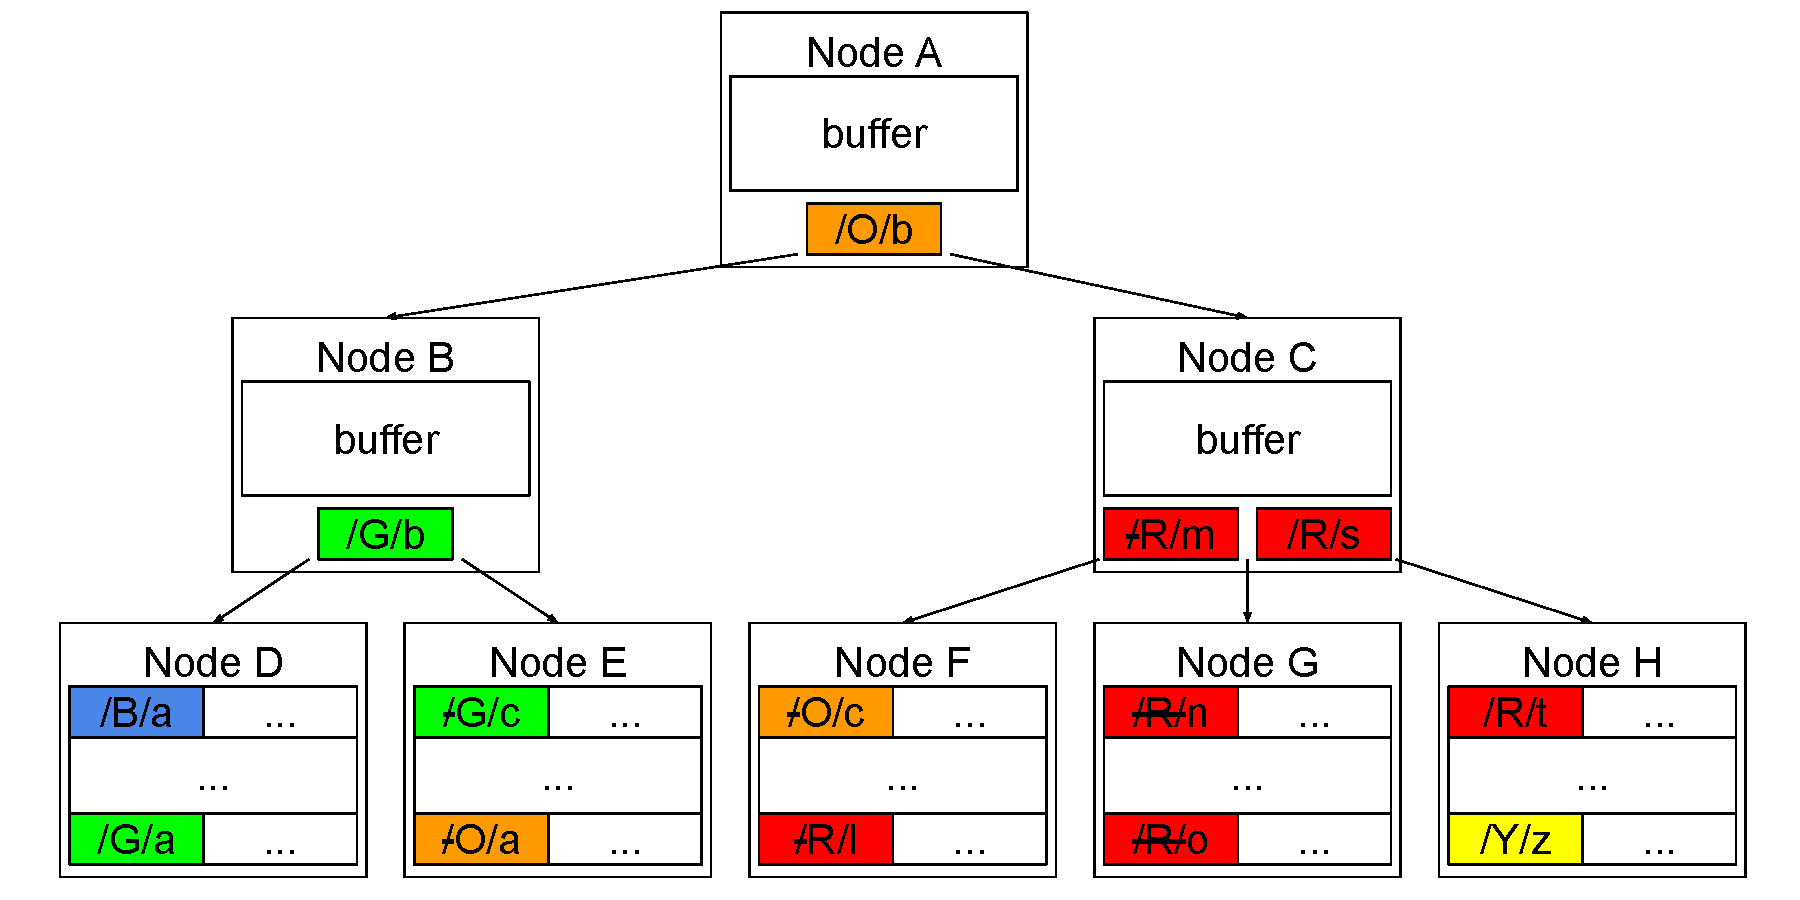
\includegraphics[width=.7\linewidth]{fig/rr-1}
        \caption{\label{subfig:rc1-1} The \bet before the range-clone.}
    \end{subfigure}
    \begin{subfigure}{\textwidth}
        \centering
        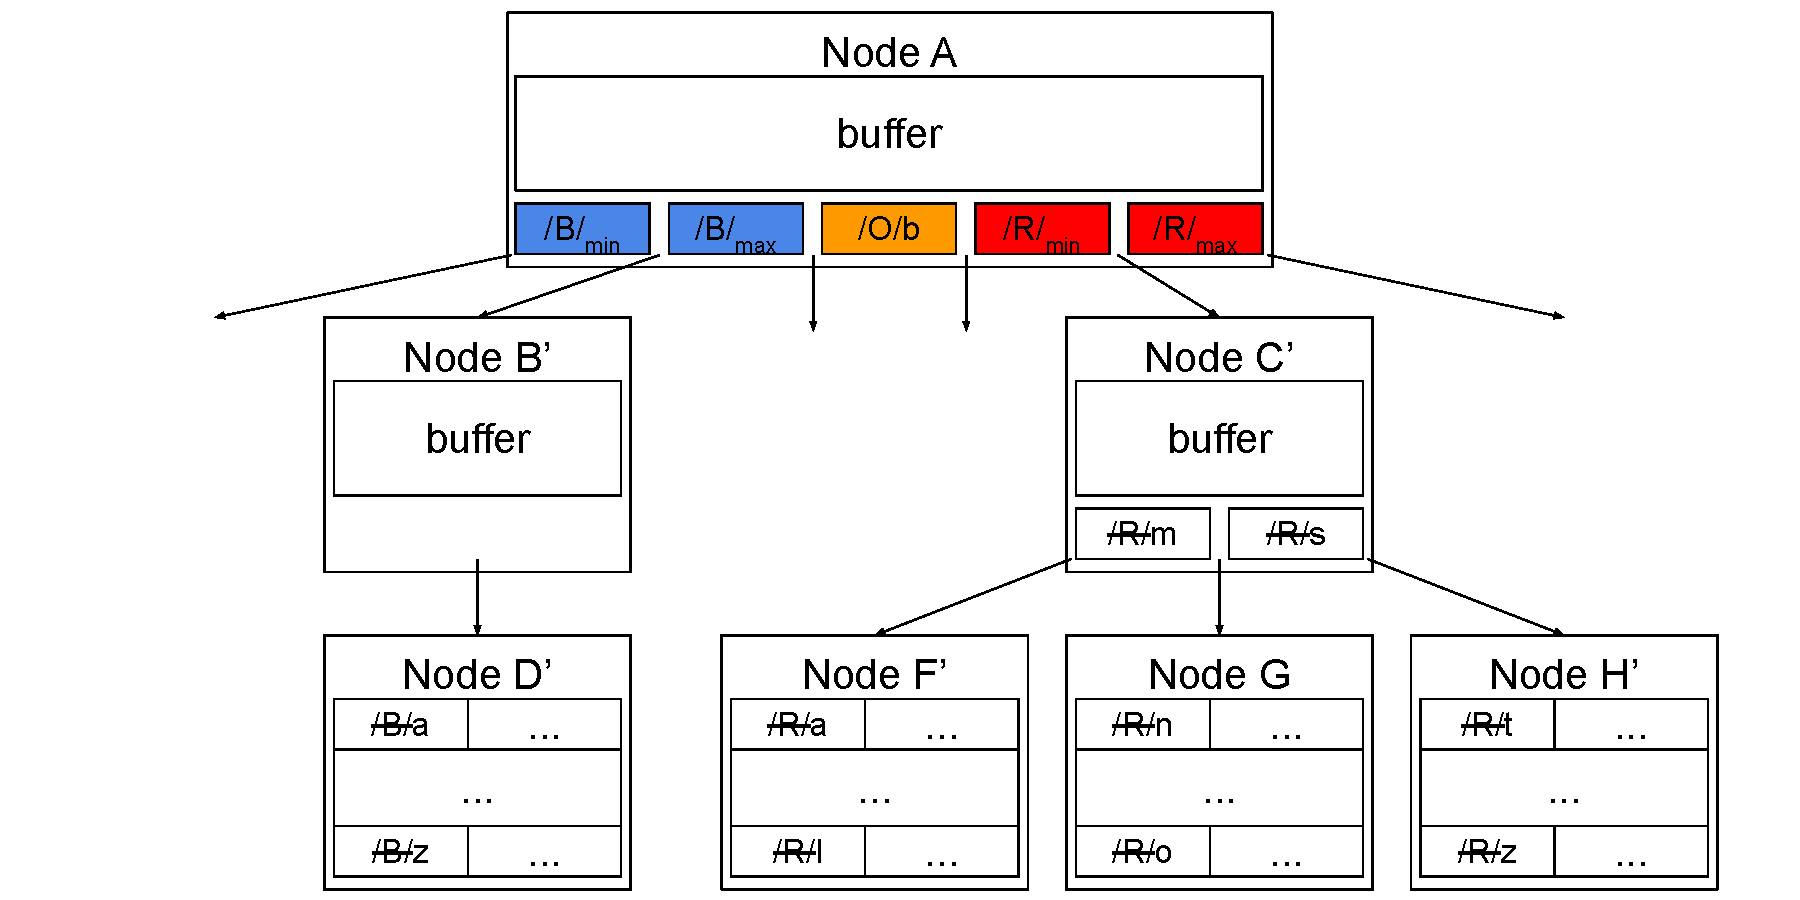
\includegraphics[width=.7\linewidth]{fig/rr-2}
        \caption{\label{subfig:rc1-2} The range-clones performs tree surgery
            to slices out the source and destination subtrees.}
    \end{subfigure}
    \begin{subfigure}{\textwidth}
        \centering
        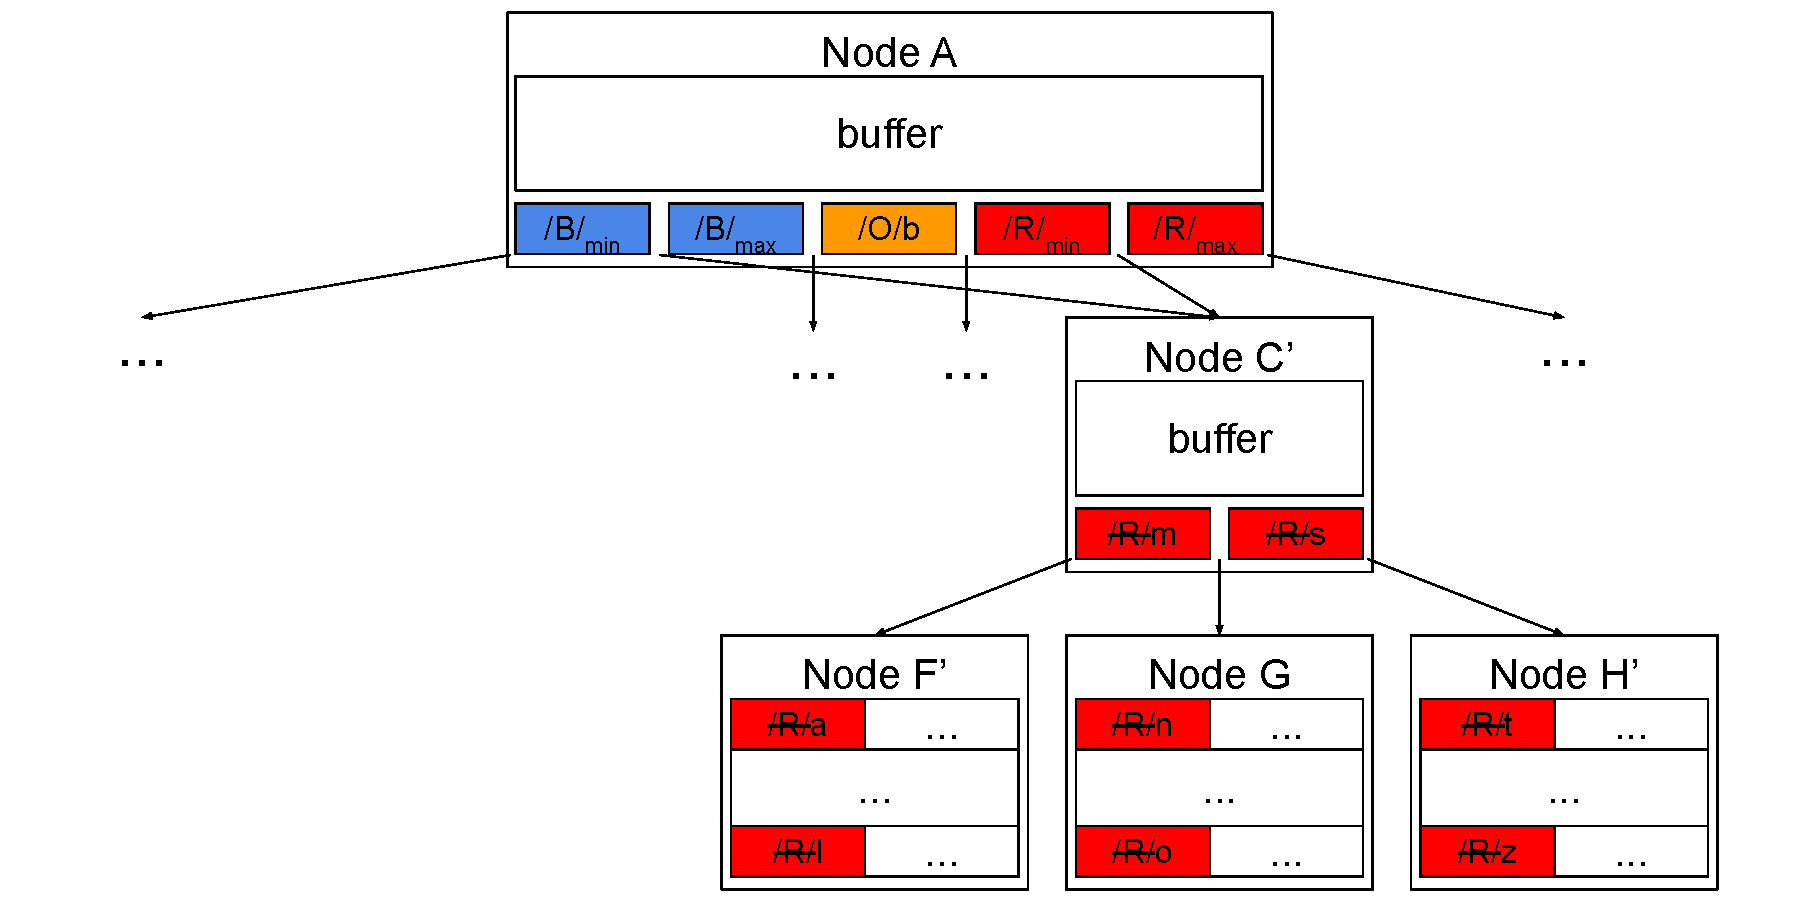
\includegraphics[width=.7\linewidth]{fig/rc1-3}
        \caption{\label{subfig:rc1-3} The range-clone discards the destination
            subtree and shares the source subtree.}
    \end{subfigure}
    \caption[A range-clone example using range-rename code]{\label{fig:rc1}
        An example of range-clone(``/R/'', ``/B/''), implemented with
        range-rename operations.}
\end{figure}

\subsection{Write-optimized tree surgery}

\subsection{\goto messages}

\section{Preferential splitting}
